\section{Permutasjoner}

\begin{definition}{Permutasjon}{}
	En \textbf{permutasjon} av en mengde $A$ er en bijeksjon $A\ra A$
\end{definition}

\textbf{Eksempler}:
\begin{enumerate}
	\item Bijeksjonen $\sigma : \mathbb{Z} \ra \mathbb{Z}$ gitt ved $\sigma(n)=-n$
	\item Bijeksjonen $\sigma : \mathbb{Z} \ra \mathbb{Z}$ gitt ved $\sigma(n)=n+a$ hvor
	      $a\in \mathbb{Z}$ er fiksert
\end{enumerate}

\textbf{Notasjon}: Dersom $A=\cb{1, \dots, n}$ og $\sigma : A\ra A$ er en permutasjon så skriver
vi følgende:
\begin{align}
	\begin{pmatrix} 1 & 2 & \cdots & n \\ \sigma(1) & \sigma(2) & \cdots & \sigma(n) \end{pmatrix}
\end{align}

\textbf{Eksempel}: Dersom vi har $A=\cb{1, 2, 3, 4}$ og $\sigma : A\ra A$ er en permutasjon med
\begin{align}
	\sigma(1) & =3 \\
	\sigma(2) & =2 \\
	\sigma(3) & =4 \\
	\sigma(4) & =1
\end{align}
Så skriver vi
\begin{align}
	\begin{pmatrix} 1 & 2 & 3 & 4 \\ 3 & 2 & 4 & 1 \end{pmatrix}
\end{align}

\textbf{Merk}: Komposisjon av to permutasjoner, $\tau, \sigma : A \ra A$ gir oss en ny permutasjon
$\tau\sigma(a):A\ra A$, definert som
\begin{align}
	\tau\sigma(a)= \tau(\sigma(a))\ \forall a\in A
\end{align}

\textbf{Eksempel}: For følgende permutasjoner,
\begin{align}
	\sigma & = \begin{pmatrix} 1 & 2 & 3 & 4 \\ 3 & 2 & 4 & 1 \end{pmatrix}  \\
	\tau   & = \begin{pmatrix} 1 & 2 & 3 & 4 \\ 2 & 1 & 4 & 3 \end{pmatrix},
\end{align}
hvor $A=\cb{1, 2, 3, 4}$ så har vi at
\begin{align}
	\tau\sigma & =\begin{pmatrix} 1 & 2 & 3 & 4 \\ 3 & 2 & 4 & 1 \end{pmatrix}
	\begin{pmatrix} 1 & 2 & 3 & 4 \\ 2 & 1 & 4 & 3 \end{pmatrix}               \\
	           & = \begin{pmatrix} 1 & 2 & 3 & 4 \\ 4 & 1 & 3 & 2\end{pmatrix}
\end{align}

\begin{theorem*}{}{}
	La $A\neq \emptyset$ være en vilkærlig mengde og
	\begin{align}
		S_A=\cb{\sigma:A\ra A\mid\sigma \text{ er en permutasjon}}
	\end{align}
	Da er $S_A$ en gruppe med komposisjon som binæroperasjon.
\end{theorem*}
\textbf{Bevis}: Siden $A$ er en ikke-tom mengde så er ogsa $S_A$ en ikke-tom mengde. Det følger
fra definisjonen av komposisjon at $S_A$ må være lukket under komposisjon.
\begin{enumerate}[label=$\mathscr{G}$\arabic*)]
	\item Det er kjent at komposisjon av funksjoner alltid er assosiativt
	\item Dersom vi definerer $I: A\ra A, I(a)=a$ så vil
	      $I\sigma=\sigma=\sigma I\ \forall \sigma\in A$. Altså er $I$ et gyldig identitetselement
	\item La $\sigma\in S_A$ og ta $a\in A$. Siden $\sigma$ er surjektiv så må det finnes en
	      $b\in A$ slik at $\sigma(b)=a$. Siden $\sigma$ er injektiv, så må $b$ være unik.

	      Definer $\sigma^{-1}:A\ra A$ med $\sigma^{-1}(a)=b$. Gjør dette med alle $a\in A$ for
	      den valgte permutasjonen $\sigma$, så vil $\sigma\sigma^{-1}=\sigma^{-1}\sigma=I$, som
	      betyr at $\sigma^{-1}$ er inversen til $\sigma$. \qed
\end{enumerate}

\begin{definition}{}{}
	Når $A=\cb{1, \cdots, n}$ så skriver vi $S_n$, som kalles den
	\textbf{$\mathbf{n}$'te symmetriske gruppen}
\end{definition}

\textbf{Merk}:
\begin{enumerate}
	\item $\abs{S_n}=n!$
	\item For $n\geq 3$ så er ikke $S_n$ abelsk (vis).
\end{enumerate}

\begin{theorem*}{Cayley}{}
	Enhver gruppe er isomorf med en undergruppe av $S_A$ for en mengde $A$.
\end{theorem*}

\subsection{Gruppen $S_3$}
Vi kan tolke $S_3$ som symmetrigruppen til et likesidet triangel. En illustrasjon av dette kan
ses i \autoref{fig:symmetry-group-s3}.

\begin{figure}[ht]
	\centering
	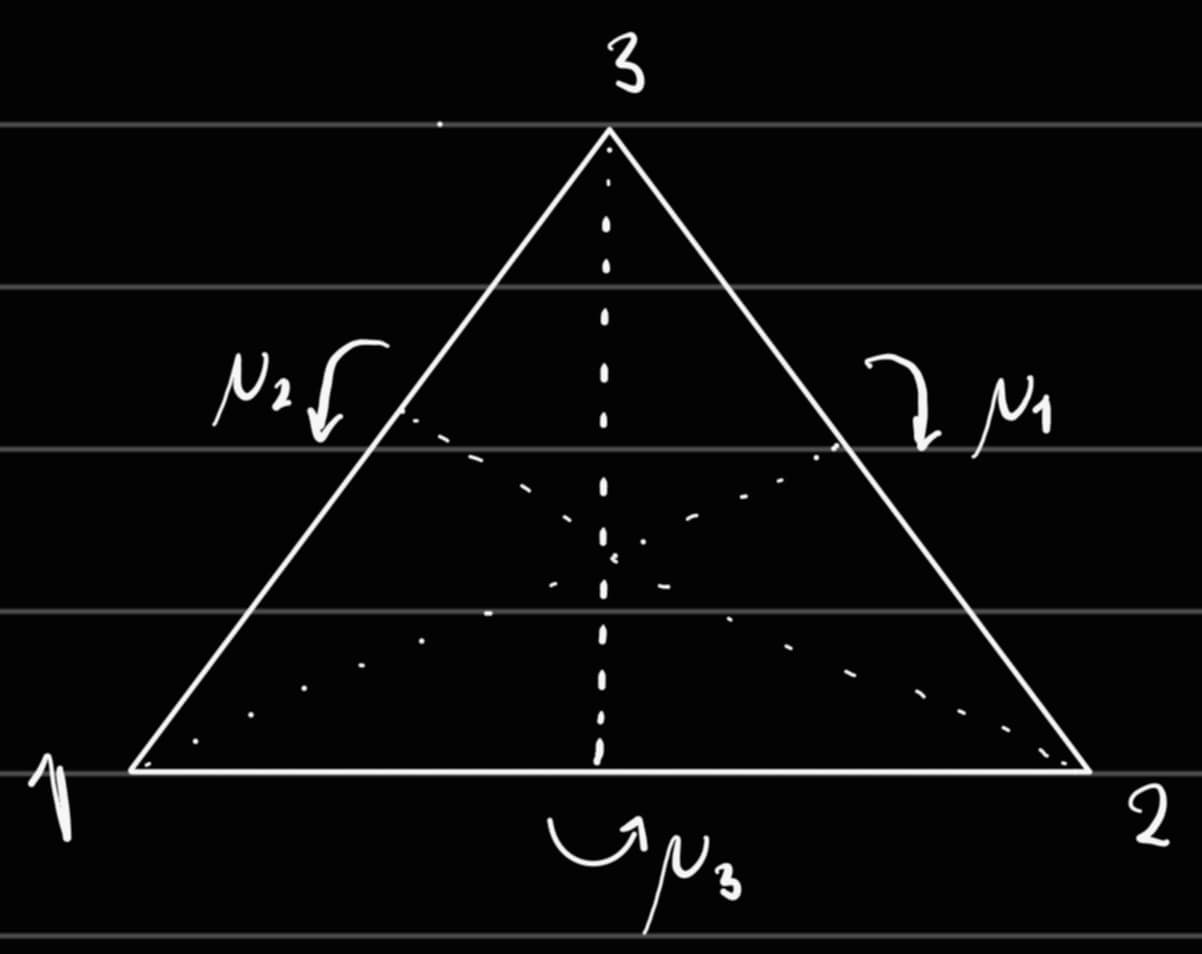
\includegraphics[width=0.5\textwidth]{images/symmetry_group_s3_illustration.jpg}
	\caption{Illustrasjon av $S_3$}
	\label{fig:symmetry-group-s3}
\end{figure}

Her definerer vi følgende elementer:
\begin{itemize}
	\item $\rho_0$: Rotasjon med $0^\circ$ mot klokken, som tilsvarer
	      $\begin{pmatrix}1 & 2 & 3 \\ 1 & 2 & 3\end{pmatrix}$
	\item $\rho_1$: Rotasjon med $120^\circ$ mot klokken, som tilsvarer
	      $\begin{pmatrix}1 & 2 & 3 \\ 2 & 3 & 1\end{pmatrix}$
	\item $\rho_2$: Rotasjon med $240^\circ$ mot klokken, som tilsvarer
	      $\begin{pmatrix}1 & 2 & 3 \\ 3 & 1 & 2\end{pmatrix}$
	\item $\mu_1$: Speiling om linje 1, som tilsvarer
	      $\begin{pmatrix}1 & 2 & 3 \\ 1 & 3 & 2\end{pmatrix}$
	\item $\mu_2$: Speiling om linje 2, som tilsvarer
	      $\begin{pmatrix}1 & 2 & 3 \\ 3 & 2 & 1\end{pmatrix}$
	\item $\mu_3$: Speiling om linje 3, som tilsvarer
	      $\begin{pmatrix}1 & 2 & 3 \\ 2 & 1 & 3\end{pmatrix}$
\end{itemize}

Binæroperasjonen i $S_3$ er komposisjon av permutasjoner, men dette svarer til komposisjon av
symmetrier.

\textbf{Eksempel}:
Vi har at
\begin{align}
	\mu_3\rho_2 & =\begin{pmatrix}1 & 2 & 3 \\ 2 & 1 & 3\end{pmatrix}
	\begin{pmatrix}1 & 2 & 3 \\ 3 & 1 & 2\end{pmatrix}                 \\
	            & = \begin{pmatrix}1 & 2 & 3 \\ 3 & 2 & 1\end{pmatrix} \\
	            & = \mu_2
\end{align}

\subsubsection{Multiplikasjonstabell til $S_3$}
Følgende er multiplikasjonstabellen til den tredje symmetrigruppen:

\[
	\begin{array}{c||cccccc}
		*      & \rho_0 & \rho_1 & \rho_2 & \mu_1 & \mu_2 & \mu_3 \\
		\hline\hline
		\rho_0 & \rho_0 & \rho_1 & \rho_2 & \mu_1 & \mu_2 & \mu_3 \\
		\rho_1 & \rho_1 & \rho_2 & \rho_0 & \mu_3 & \mu_1 & \mu_2 \\
		\rho_2 & \rho_2 & \rho_0 & \rho_1 & \mu_2 & \mu_3 & \mu_1 \\
		\mu_1  & \mu_1 & \mu_2 & \mu_3 & \rho_0 & \rho_1 & \rho_2 \\
		\mu_2  & \mu_2 & \mu_3 & \mu_1 & \rho_2 & \rho_0 & \rho_1 \\
		\mu_3  & \mu_3 & \mu_1 & \mu_2 & \rho_1 & \rho_2 & \rho_0 \\
	\end{array}
\]

\textbf{Undergrupper}:
\begin{itemize}
  \item $\cb{\rho_0}$
  \item $\cb{\rho_0, \rho_1, \rho_2}=\inner{\rho_1}=\inner{\rho_2}$
  \item $\cb{\rho_0, \mu_i}_{i=1,2,3}$
  \item $S_3$ selv, som ikke er syklisk
\end{itemize}
